\documentclass[11pt]{article}

\usepackage[review]{acl}

\usepackage{times}
\usepackage{latexsym}
\usepackage[T1]{fontenc}
\usepackage[utf8]{inputenc}
\usepackage{microtype}
\usepackage{inconsolata}
\usepackage{graphicx}
\usepackage{amsmath}
\usepackage{amssymb}
\usepackage{booktabs}
\usepackage{multirow}
\usepackage{array}
\usepackage{subcaption}

\title{Detecting Hallucinations in Large Language Models via Attention-Head-Level Probes and Voting Ensembles}

\author{
  Luyu Lu \\
  School of Computer Science \\
  \texttt{231880506@stu.edu.cn} \\\And
  Shengwen Liu \\
  School of Computer Science \\
  \texttt{231880321@stu.edu.cn} \\}

\begin{document}
\maketitle

\begin{abstract}
Large language models (LLMs) are prone to generating factually incorrect text---so-called \emph{hallucinations}---often accompanied by high confidence. We investigate hallucination detection methods that leverage the model's internal states without requiring external knowledge retrieval. Using Qwen2-1.5B (28-layer Transformer, 12 heads per layer, hidden size 1536), we conduct a systematic three-stage study. First, we establish baselines comparing perplexity (PPL) and SAPLMA (probe on hidden states), finding that SAPLMA achieves an average AUC of 0.834 versus 0.690 for PPL on a six-topic true/false dataset. Second, we analyze the roles of layer depth and token position, confirming that the middle-upper layers (especially Layer 18) and the last token position carry the richest discriminative signals. Third, we propose a novel per-head probe method: training independent binary classifiers on each of the 336 attention heads' influence vectors, selecting the top-5 heads by validation AUC, and combining them via a voting ensemble. On a TriviaQA-based test set (203 samples), the summed-heads probe achieves AUC 0.776, surpassing the full SAPLMA baseline (AUC 0.723) with only 5 of 336 heads. The most discriminative heads cluster in layers 13--16, consistent with SAPLMA's optimal layer range. Our results demonstrate that interpretable, head-level probes can rival or exceed full-hidden-state methods for hallucination detection.
\end{abstract}

\section{Introduction}

Large language models have achieved remarkable performance across a wide range of natural language processing tasks. However, a persistent and critical failure mode is their tendency to generate text that appears fluent and confident but contains factual errors---a phenomenon commonly referred to as \emph{hallucination} \citep{lin2022truthfulqa, bai2022constitutional}. Hallucination poses significant risks in high-stakes applications such as medical question answering, legal consultation, and knowledge retrieval, where factual accuracy is paramount.

Existing approaches to hallucination detection can be broadly categorized into two families. \emph{Extrinsic} methods rely on external knowledge bases or retrieval systems to verify generated claims \citep{manakul2023selfcheckgpt}, incurring additional latency and infrastructure costs. \emph{Intrinsic} methods, by contrast, exploit the model's own internal representations---hidden states, attention patterns, or output probabilities---to distinguish truthful from hallucinated outputs \citep{azaria2023internal, burns2022discovering}. Intrinsic methods are appealing because they require no external resources and can operate in real time.

In this work, we conduct a systematic investigation of intrinsic hallucination detection methods using Qwen2-1.5B \citep{qwen2024qwen2}, a 28-layer Transformer model. Our study proceeds in three stages:

\begin{enumerate}
    \item \textbf{Baseline Comparison} (Section~\ref{sec:baseline}): We reproduce and compare two established methods---perplexity-based detection (PPL) and SAPLMA \citep{azaria2023internal}---on a six-topic true/false dataset, establishing that SAPLMA (average AUC 0.834) significantly outperforms PPL (average AUC 0.690).
    \item \textbf{Representation Analysis} (Section~\ref{sec:analysis}): We investigate how layer depth and token position affect detection quality, confirming an inverted-U performance curve peaking at Layer 18 and demonstrating that the last token position is critical for detection.
    \item \textbf{Per-Head Probe Method} (Section~\ref{sec:headprobe}): We propose a novel approach that trains independent binary classifiers on individual attention heads' influence vectors, selects the top-5 most discriminative heads by validation AUC, and combines them via a voting ensemble. This method achieves AUC 0.776 on a TriviaQA test set using only 5 of 336 heads, surpassing the full SAPLMA baseline.
\end{enumerate}

Our key contribution is demonstrating that interpretable, head-level probes can rival or exceed full-hidden-state methods for hallucination detection, while revealing which specific attention heads are most responsible for encoding the model's ``knowledge'' of factual correctness.

\section{Related Work}

\paragraph{Internal Representations of Truth.} \citet{azaria2023internal} showed that a probe trained on the hidden states of an LLM can predict whether a statement is true or false, achieving significantly better performance than perplexity-based methods. \citet{marks2023geometry} demonstrated that true/false representations exhibit emergent linear structure in LLM hidden states. \citet{li2023inference} proposed inference-time interventions to elicit truthful answers by manipulating internal representations.

\paragraph{Unsupervised Probes.} \citet{burns2022discovering} introduced Contrast-Consistent Search (CCS), an unsupervised method for extracting truth-direction representations from LLM hidden states without labeled data, using contrast pairs and a consistency/informativeness loss.

\paragraph{Attention Head Analysis.} \citet{clark2019bert} analyzed BERT's attention patterns to understand what linguistic information different heads capture. \citet{elhage2022toy} and \citet{olah2020zoom} developed frameworks for understanding neural network circuits, including the role of individual attention heads in information processing. \citet{meng2022locating} demonstrated that factual knowledge is localized in specific model components, motivating our per-head analysis.

\paragraph{Hallucination Detection.} \citet{manakul2023selfcheckgpt} proposed SelfCheckGPT for zero-resource hallucination detection. \citet{wei2024simple} showed that synthetic data can reduce sycophantic behavior in LLMs. Our work focuses on the intrinsic detection paradigm, extending SAPLMA to the attention-head level.

\section{Methodology}
\label{sec:methodology}

\subsection{Model and Datasets}
\label{sec:setup}

\paragraph{Model.} We use Qwen2-1.5B \citep{qwen2024qwen2}, a causal language model with 28 Transformer layers, 12 attention heads per layer, head dimension 128, and hidden size $d_{\text{model}} = 1536$. The model totals 336 attention heads.

\paragraph{True-False Dataset.} Following \citet{azaria2023internal}, we use a dataset of true/false statements spanning six topics: Cities, Inventions, Chemical Elements, Animals, Companies, and Scientific Facts. Each topic contains paired true and false statements.

\paragraph{TriviaQA Dataset.} For Stage 3, we sample questions from TriviaQA \citep{joshi2017triviaqa}, generate answers using Qwen2-1.5B with greedy decoding, and auto-label them as correct or hallucinated via fuzzy substring matching against the provided ideal answer aliases.

\subsection{Stage 1: Baseline Methods}
\label{sec:baseline}

\subsubsection{Perplexity-Based Detection (PPL)}

The PPL method is parameter-free: for each statement, we compute the negative log-likelihood (NLL):
\begin{equation}
    \text{NLL}(x) = -\frac{1}{T} \sum_{t=1}^{T} \log p(x_t \mid x_{<t})
\end{equation}
where $T$ is the sequence length. Higher NLL indicates the model considers the statement less probable, suggesting a hallucination. An optimal threshold is found by maximizing accuracy on the ROC curve.

\subsubsection{SAPLMA: Probe on Hidden States}

SAPLMA \citep{azaria2023internal} extracts the last token's hidden state from intermediate layers and trains a supervised probe. We extract embeddings from layers 14, 18, 22, 26, and 28 (every 4 layers from the middle to the last layer) and train a three-layer feedforward probe:
\begin{equation}
    \text{Probe}(h) = \sigma(W_3 \cdot \text{ReLU}(W_2 \cdot \text{ReLU}(W_1 \cdot h + b_1) + b_2) + b_3)
\end{equation}
with layer dimensions 256$\to$128$\to$64$\to$1, ReLU activations, sigmoid output, Adam optimizer, and binary cross-entropy loss. We use leave-one-out cross-validation (5 topics train, 1 topic tests) with 3 random restarts per configuration and 5 training epochs.

\subsection{Stage 2: Representation Analysis}
\label{sec:analysis}

\subsubsection{Layer Depth Analysis}

We evaluate SAPLMA probes at layers 14, 18, 22, 26, and 28 to characterize how detection quality varies with depth. This reveals the optimal layer for extracting truth-discriminative representations.

\subsubsection{Token Position Analysis}

At Layer 18 (the optimal layer), we compare probe performance using hidden states from four token positions:
\begin{itemize}
    \item \textbf{First} (position 0): The beginning of the statement.
    \item \textbf{Second} (position 1): The second token.
    \item \textbf{Second-to-Last} (position $-2$): The penultimate token.
    \item \textbf{Last} (position $-1$): The final token (default SAPLMA setting).
\end{itemize}

\subsection{Stage 3: Per-Head Probe and Voting}
\label{sec:headprobe}

\subsubsection{Influence Vector Extraction}

In a Transformer, each attention head $h$ at layer $l$ contributes an incremental vector to the residual stream:
\begin{equation}
    \Delta_h = O_h \cdot W_O^h
\end{equation}
where $O_h \in \mathbb{R}^{T \times d_{\text{head}}}$ is the attention output of head $h$, and $W_O^h \in \mathbb{R}^{d_{\text{model}} \times d_{\text{head}}}$ is the corresponding slice of the output projection matrix. The vector $\Delta_h \in \mathbb{R}^{d_{\text{model}}}$ is the \emph{influence vector} of head $h$, directly contributing to the final hidden state.

We extract influence vectors for all 336 heads by hooking the input to each layer's \texttt{o\_proj} module, slicing by head, and computing the matrix product with the corresponding weight slice. Features are taken at the answer's last token position.

\subsubsection{Head Selection via Classifier AUC}

For each of the 336 attention heads, we train an independent binary classifier (same architecture as the SAPLMA probe) on the training set (Set A, $\sim$500 samples). We evaluate each classifier's AUC on a held-out validation set (Set B, $\sim$300 samples) and select the top-5 heads by validation AUC:
\begin{equation}
    \text{Top-5} = \arg\text{top-}_{h \in \{1,\ldots,336\}} \text{AUC}_h^{\text{val}}
\end{equation}

\subsubsection{Voting Ensemble}

On the test set (Set C, 203 samples), we evaluate multiple fusion strategies:

\begin{itemize}
    \item \textbf{Single-Head Probe}: Each of the top-5 heads independently classifies via its own probe.
    \item \textbf{Summed-Heads Probe}: The influence vectors of the top-5 heads are element-wise summed into a single $d_{\text{model}}$-dimensional vector, and one probe is trained on the combined feature.
    \item \textbf{Voting Ensemble}: Each single-head probe outputs a probability; these are binarized via ROC-optimized thresholds, and the final prediction is the majority vote across the 5 probes.
\end{itemize}

\section{Experiments and Results}

\subsection{Stage 1: PPL vs SAPLMA}
\label{sec:results_stage1}

Table~\ref{tab:ppl_metrics} shows PPL performance across six topics. PPL achieves its best performance on Facts (AUC 0.775) and worst on Inventions (AUC 0.638), with an average AUC of 0.690.

\begin{table}[t]
\centering
\begin{tabular}{lccc}
\toprule
\textbf{Dataset} & \textbf{Accuracy} & \textbf{AUC} & \textbf{Threshold} \\
\midrule
Cities       & 0.703 & 0.740 & 3.969 \\
Inventions   & 0.603 & 0.638 & 5.233 \\
Elements     & 0.624 & 0.662 & 3.304 \\
Animals      & 0.624 & 0.658 & 4.318 \\
Companies    & 0.626 & 0.670 & 4.041 \\
Facts        & 0.722 & 0.775 & 2.961 \\
\midrule
\textbf{Average} & \textbf{0.650} & \textbf{0.690} & --- \\
\bottomrule
\end{tabular}
\caption{PPL-based hallucination detection results across six true/false datasets. The average AUC is 0.690.}
\label{tab:ppl_metrics}
\end{table}

Table~\ref{tab:saplma_layer} presents SAPLMA results across five layers. Layer 18 achieves the best average performance (Accuracy 0.739, AUC 0.834), while the final layer (28) performs worst (AUC 0.761), exhibiting an inverted-U pattern.

\begin{table}[t]
\centering
\begin{tabular}{lcccccc}
\toprule
\textbf{Layer} & \textbf{Cit.} & \textbf{Inv.} & \textbf{Ele.} & \textbf{Ani.} & \textbf{Com.} & \textbf{Fac.} \\
\midrule
14 & .919 & .853 & .733 & .773 & .908 & .804 \\
18 & .912 & .863 & .698 & .765 & .913 & .853 \\
22 & .903 & .775 & .774 & .775 & .878 & .834 \\
26 & .864 & .786 & .768 & .705 & .823 & .816 \\
28 & .838 & .743 & .750 & .698 & .742 & .798 \\
\midrule
\textbf{Avg} & .887 & .804 & .745 & .743 & .853 & .821 \\
\bottomrule
\end{tabular}
\caption{SAPLMA AUC by layer and topic. Layer 18 achieves the highest average AUC (0.834). Values shown are average AUC across 3 random restarts with leave-one-out cross-validation.}
\label{tab:saplma_layer}
\end{table}

Figure~\ref{fig:ppl_vs_saplma} visualizes the PPL vs SAPLMA comparison. SAPLMA outperforms PPL on every topic, with an average AUC improvement of 0.144.

\begin{figure}[t]
    \centering
    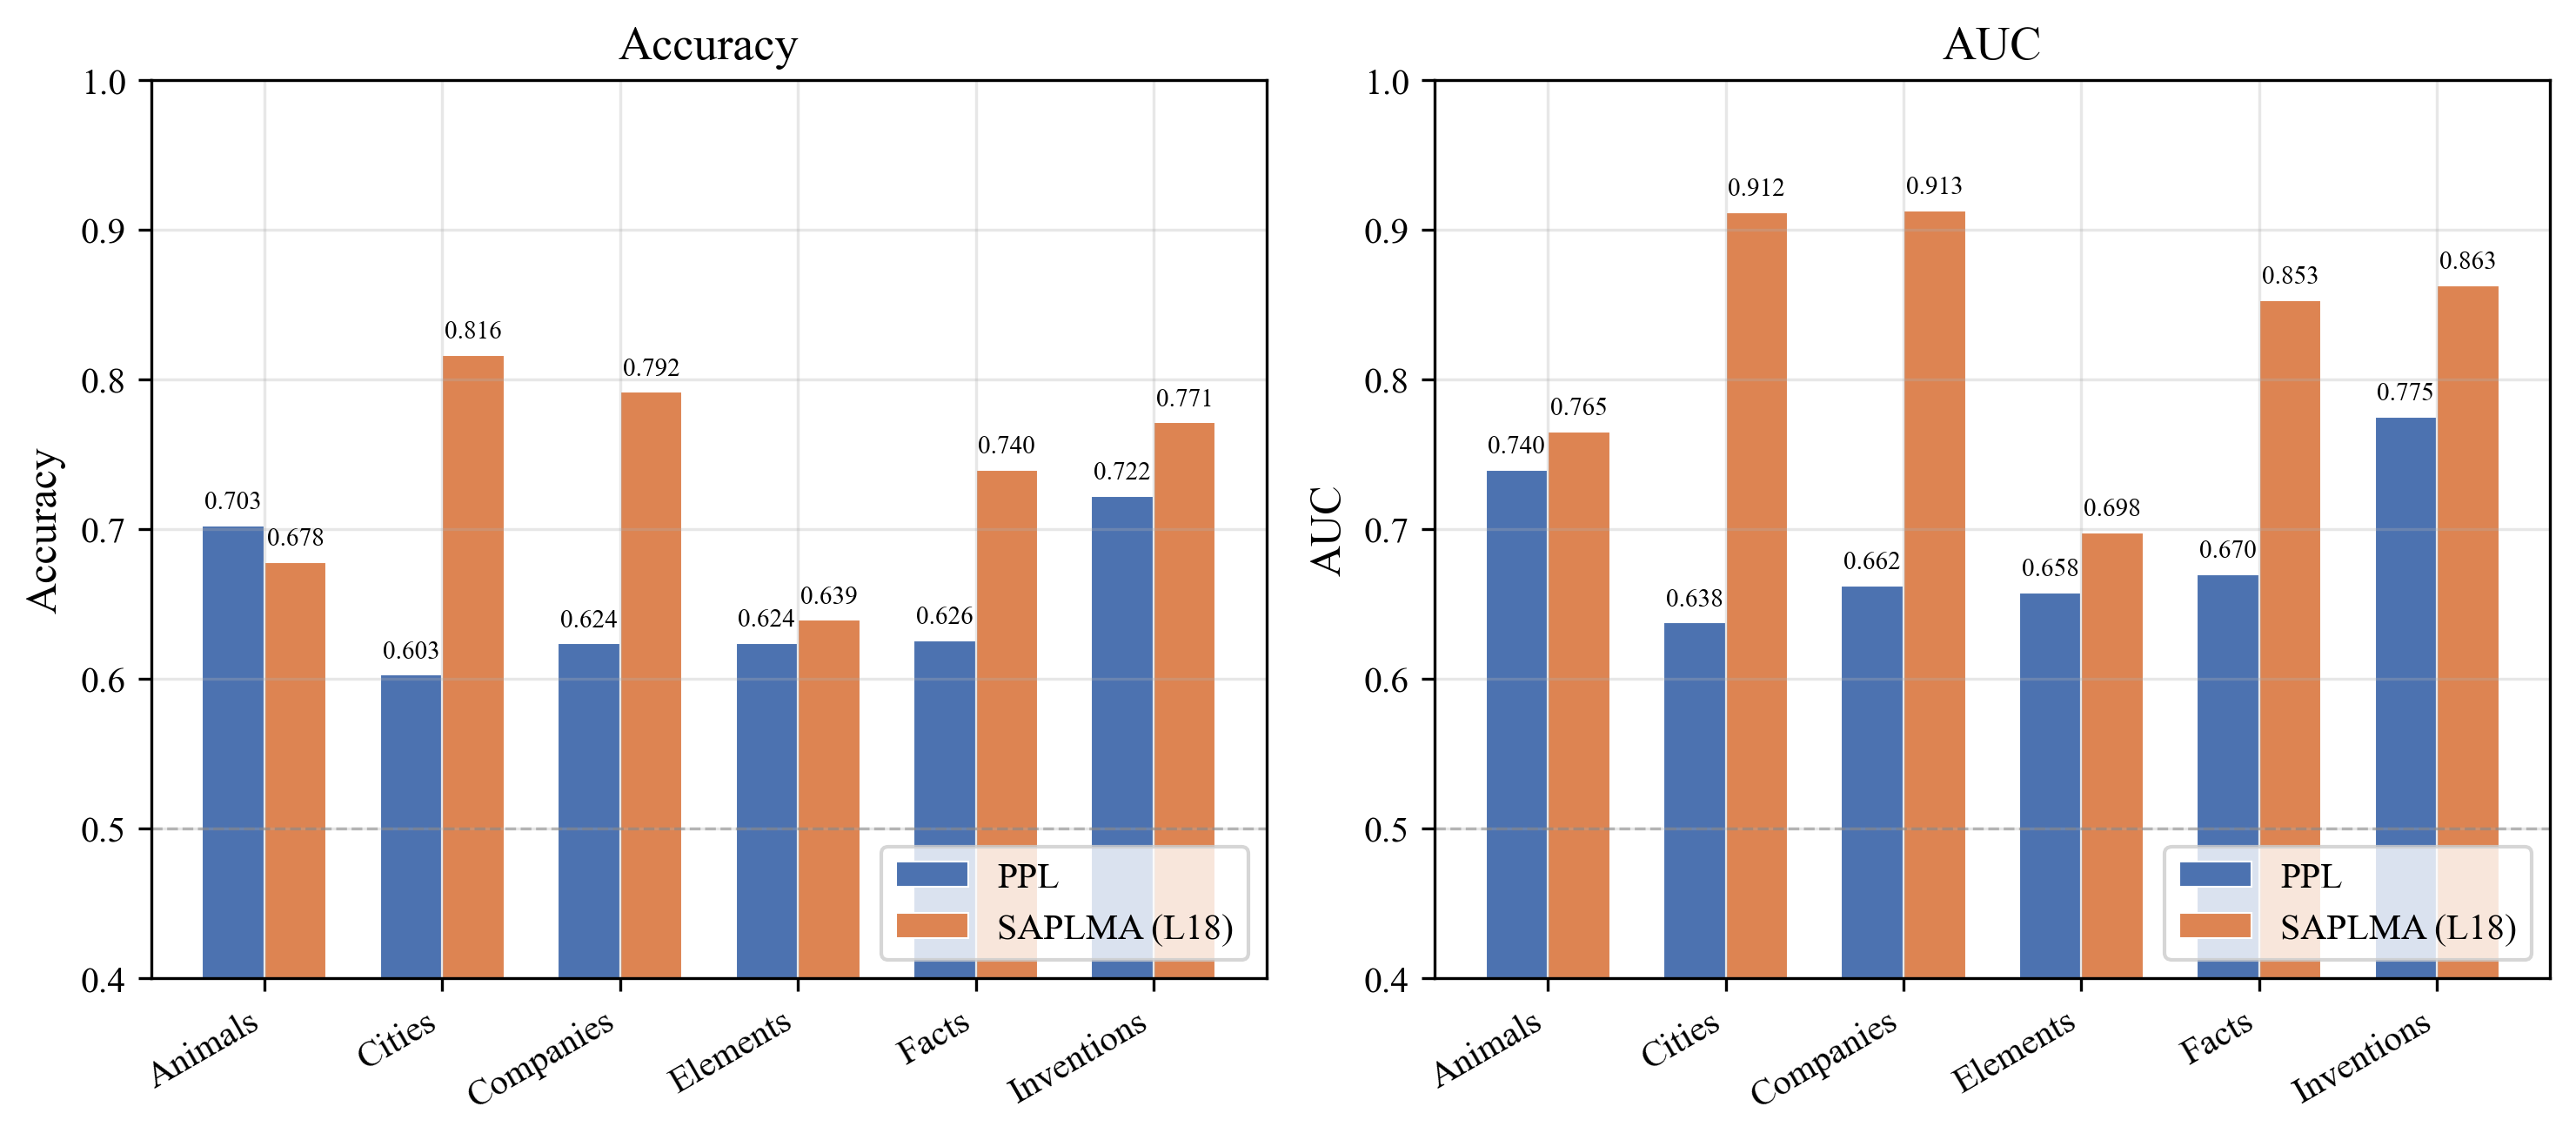
\includegraphics[width=\columnwidth]{processed_datasets/fig_report_1_ppl_vs_saplma.png}
    \caption{PPL vs SAPLMA (Layer 18) comparison across six topics. SAPLMA consistently outperforms PPL in both Accuracy and AUC.}
    \label{fig:ppl_vs_saplma}
\end{figure}

\subsection{Stage 2: Layer Depth and Token Position}
\label{sec:results_stage2}

Figure~\ref{fig:layer_analysis} shows how SAPLMA performance varies with layer depth. The left panel confirms the inverted-U pattern, with Layer 18 (64\% depth) achieving the best average AUC. The right panel shows this pattern holds across most topics, though the exact peak varies slightly.

\begin{figure}[t]
    \centering
    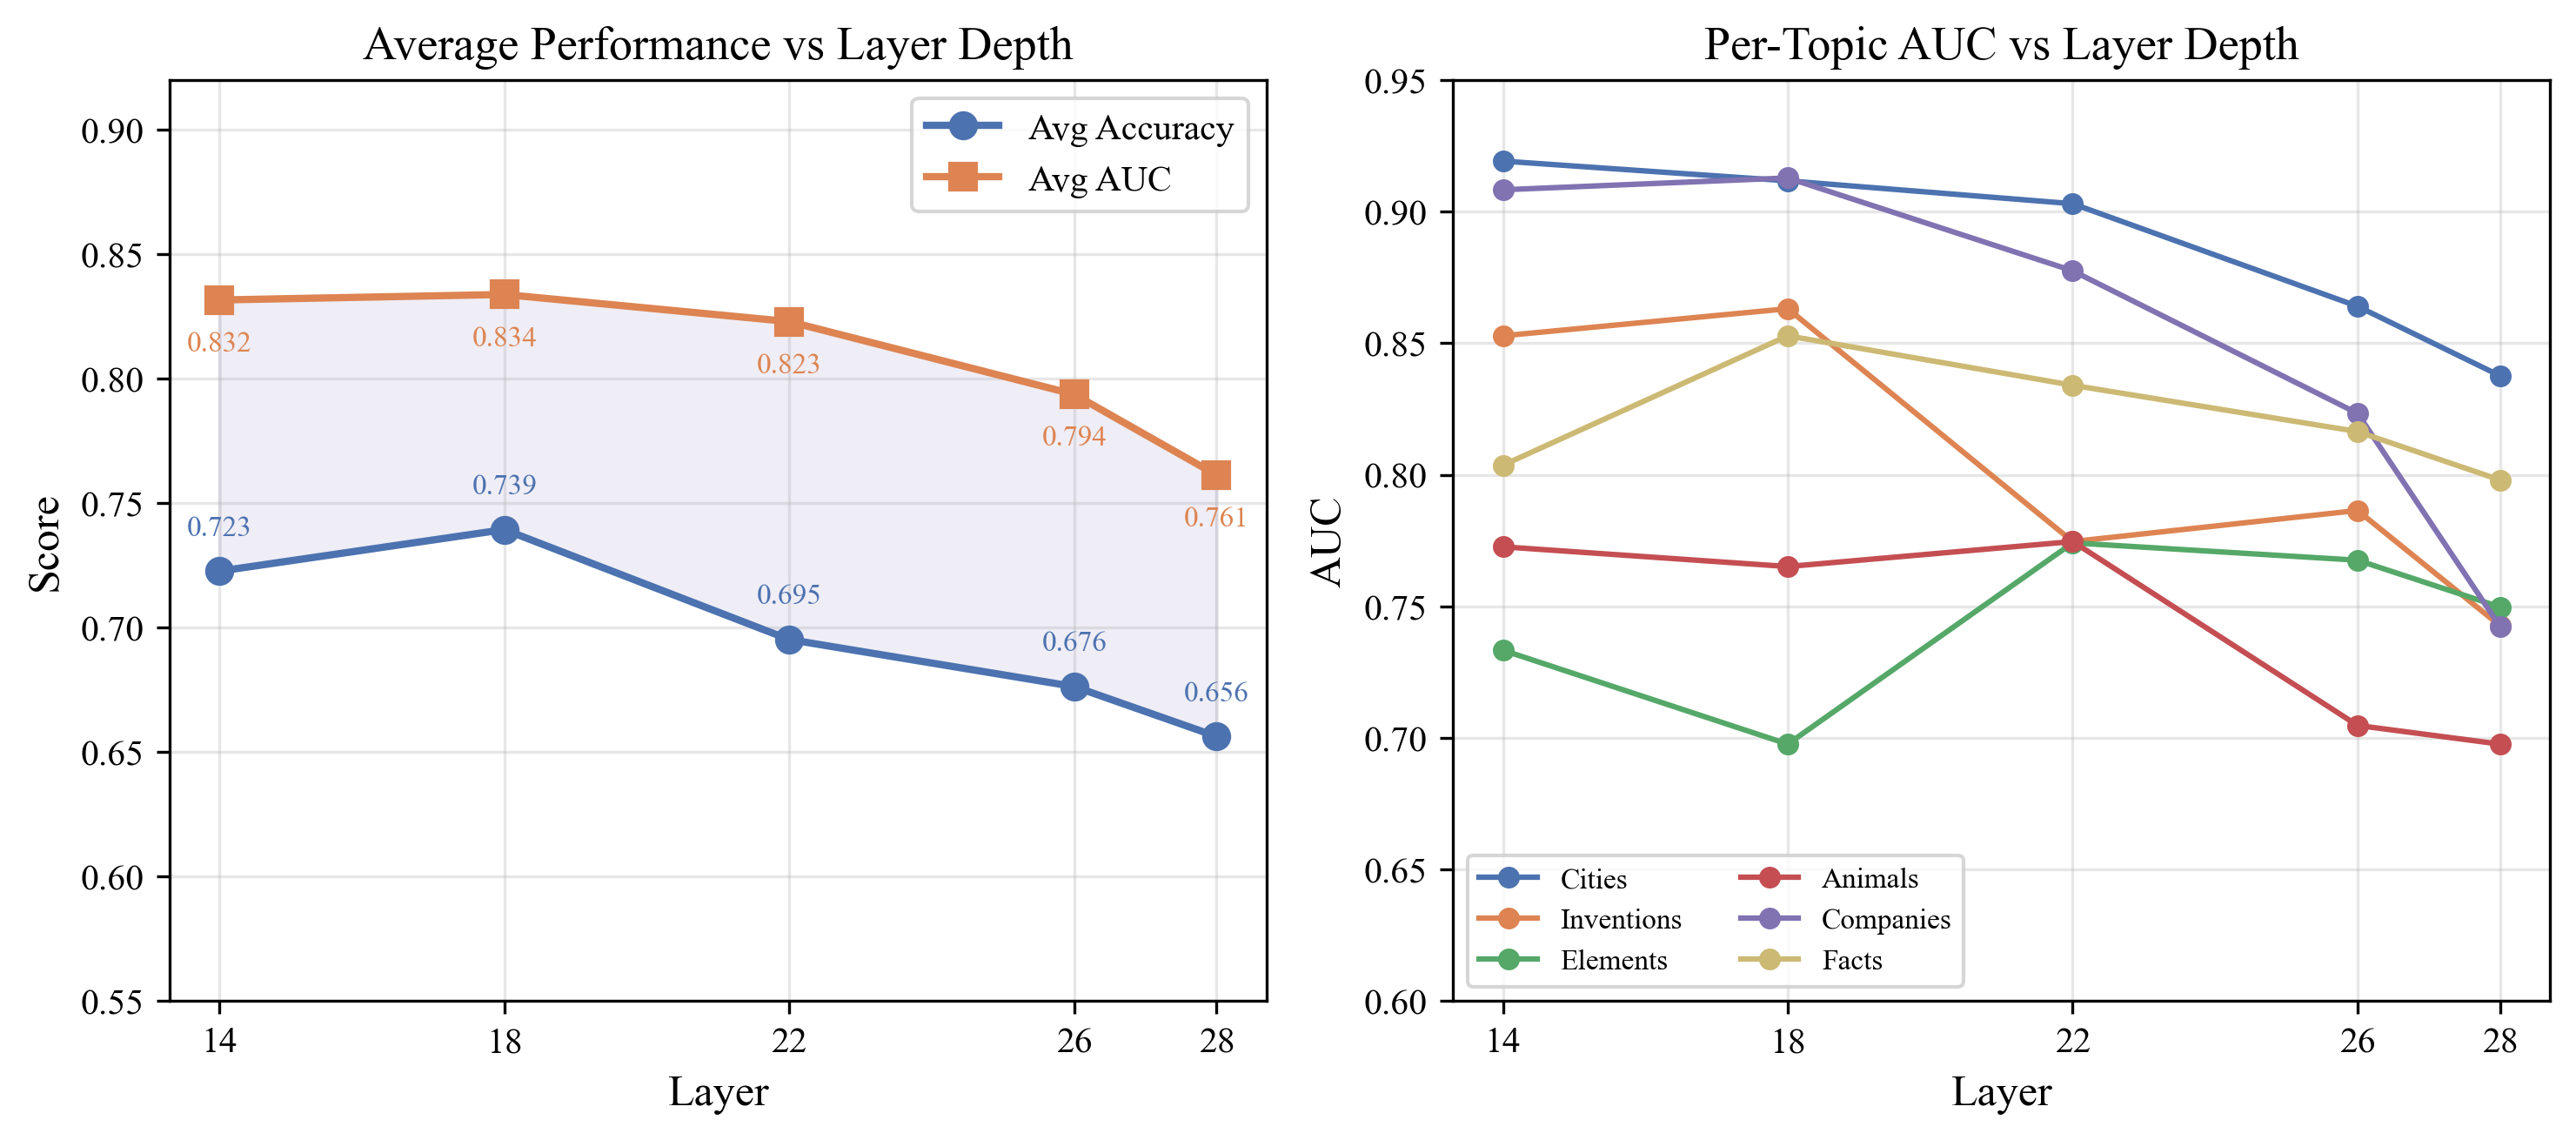
\includegraphics[width=\columnwidth]{processed_datasets/fig_report_2_layer_analysis.png}
    \caption{Left: Average Accuracy and AUC across layers. Right: Per-topic AUC across layers. The inverted-U pattern peaks at Layer 18.}
    \label{fig:layer_analysis}
\end{figure}

Table~\ref{tab:token_position} and Figure~\ref{fig:token_position} present the token position analysis. The last token dramatically outperforms all other positions (AUC 0.835), while the first and second tokens are near random (AUC $\sim$0.50). The second-to-last token shows intermediate performance (AUC 0.668), suggesting a gradual accumulation of semantic information.

\begin{table}[t]
\centering
\begin{tabular}{lcc}
\toprule
\textbf{Position} & \textbf{Avg Accuracy} & \textbf{Avg AUC} \\
\midrule
First           & 0.504 & 0.500 \\
Second          & 0.504 & 0.493 \\
Second-to-Last  & 0.603 & 0.668 \\
\textbf{Last}   & \textbf{0.741} & \textbf{0.835} \\
\bottomrule
\end{tabular}
\caption{Token position analysis at Layer 18. The last token achieves dramatically superior performance.}
\label{tab:token_position}
\end{table}

\begin{figure}[t]
    \centering
    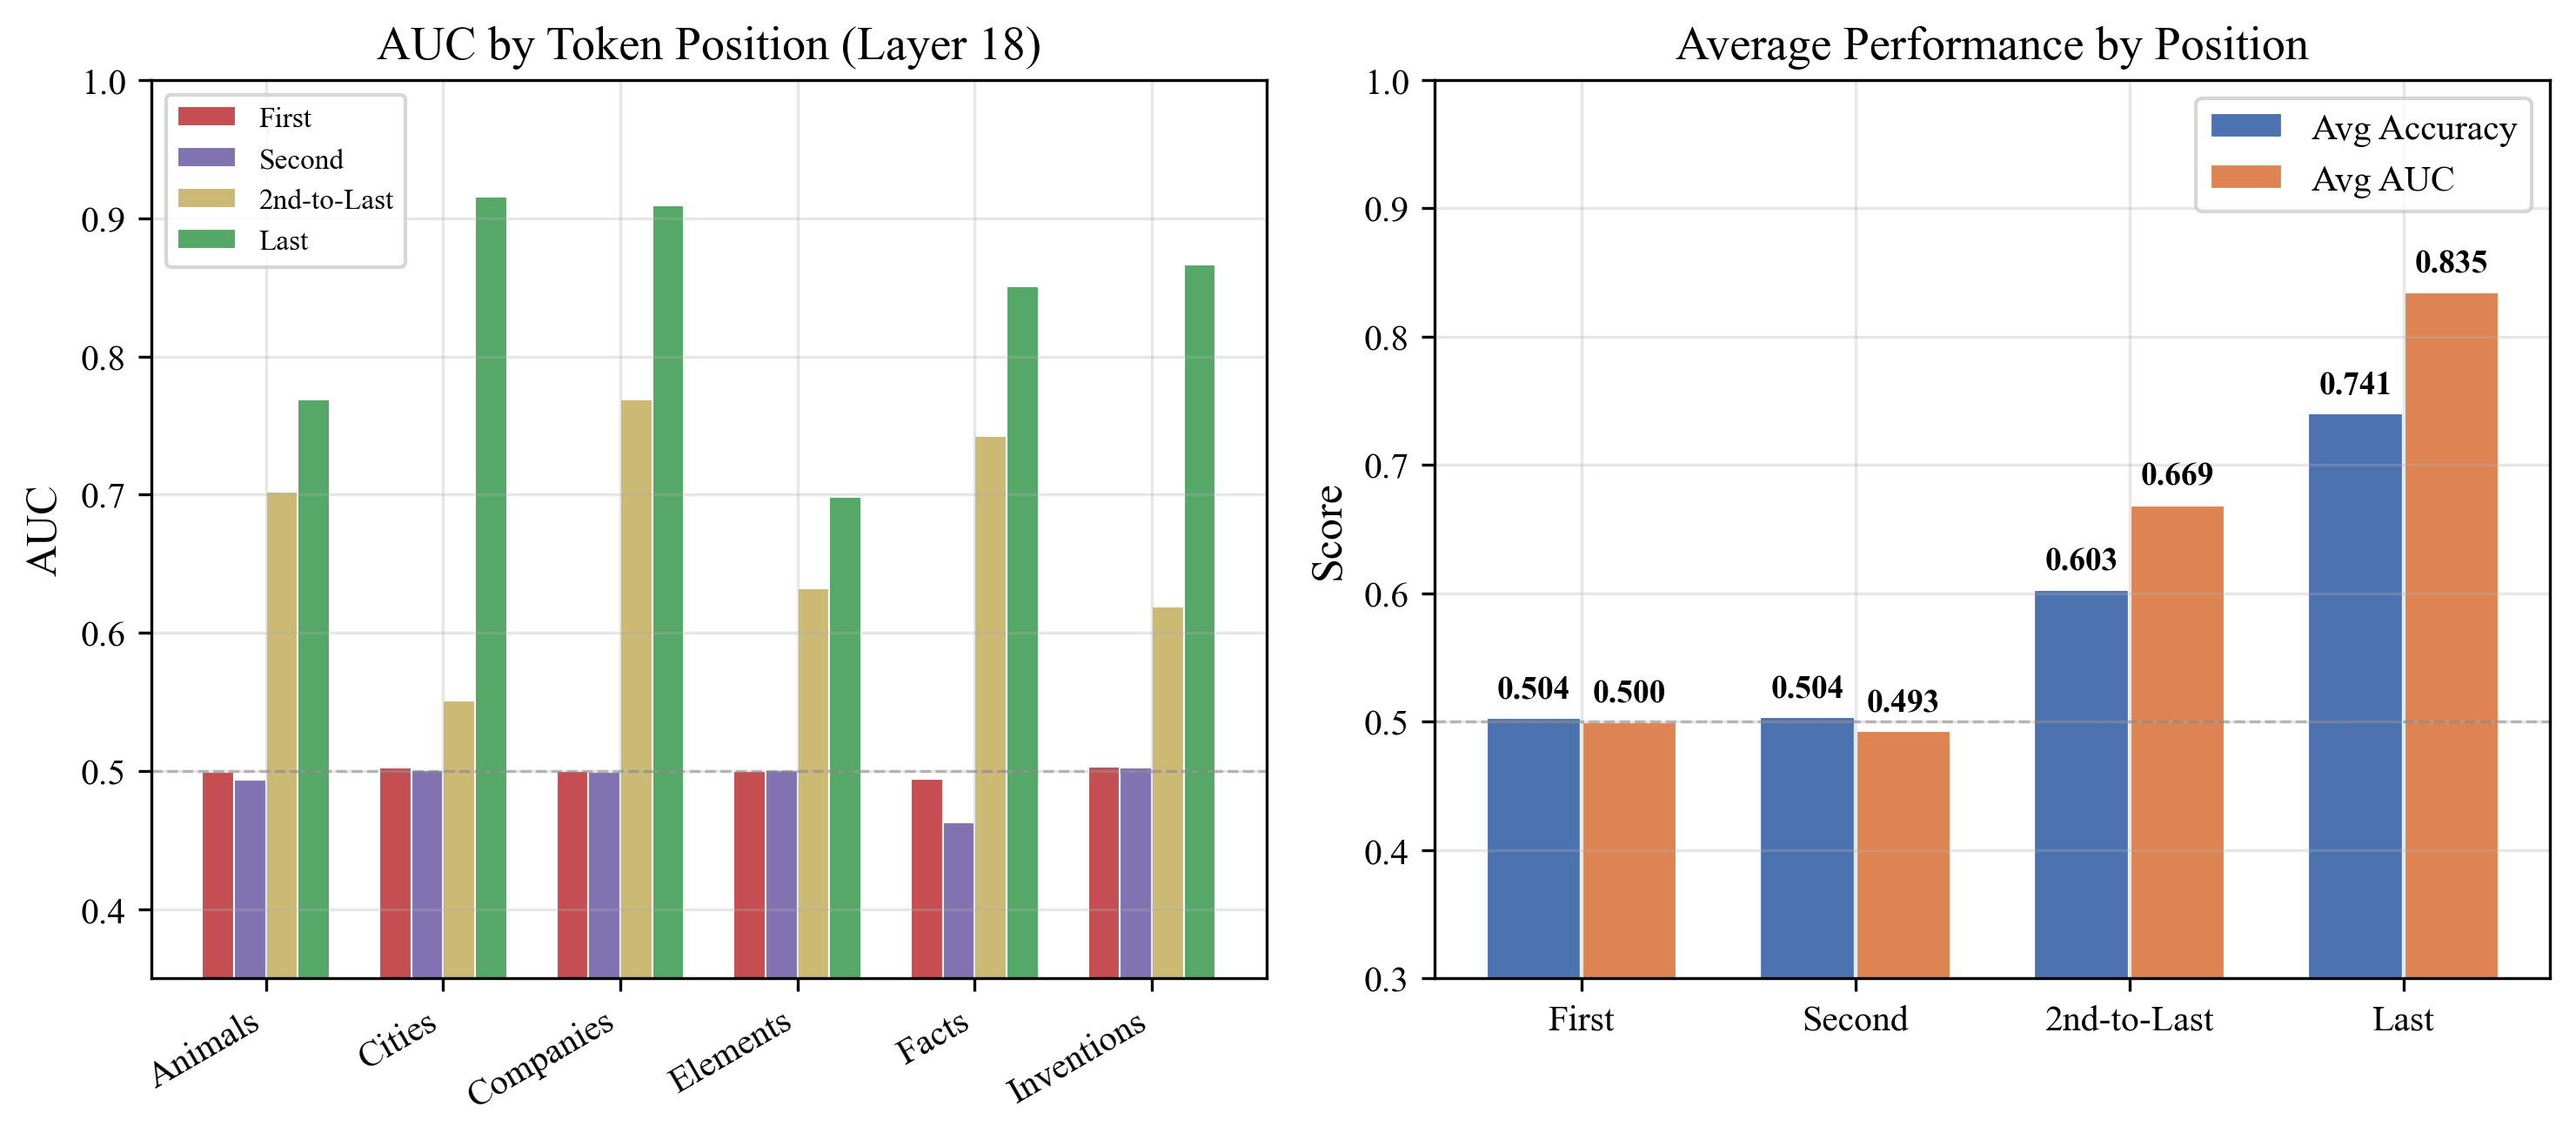
\includegraphics[width=\columnwidth]{processed_datasets/fig_report_3_token_position.png}
    \caption{Left: Per-topic AUC by token position. Right: Average performance by position. The last token is critical for hallucination detection.}
    \label{fig:token_position}
\end{figure}

\subsection{Stage 3: Per-Head Probe and Voting}
\label{sec:results_stage3}

\subsubsection{Head Selection}

We trained 336 independent binary classifiers (one per attention head) on Set A and evaluated their AUC on Set B. Figure~\ref{fig:head_heatmap} shows the AUC distribution across all heads. High-performing heads concentrate in layers 12--18, with the top head (L15\_H6) achieving AUC 0.782.

\begin{figure}[t]
    \centering
    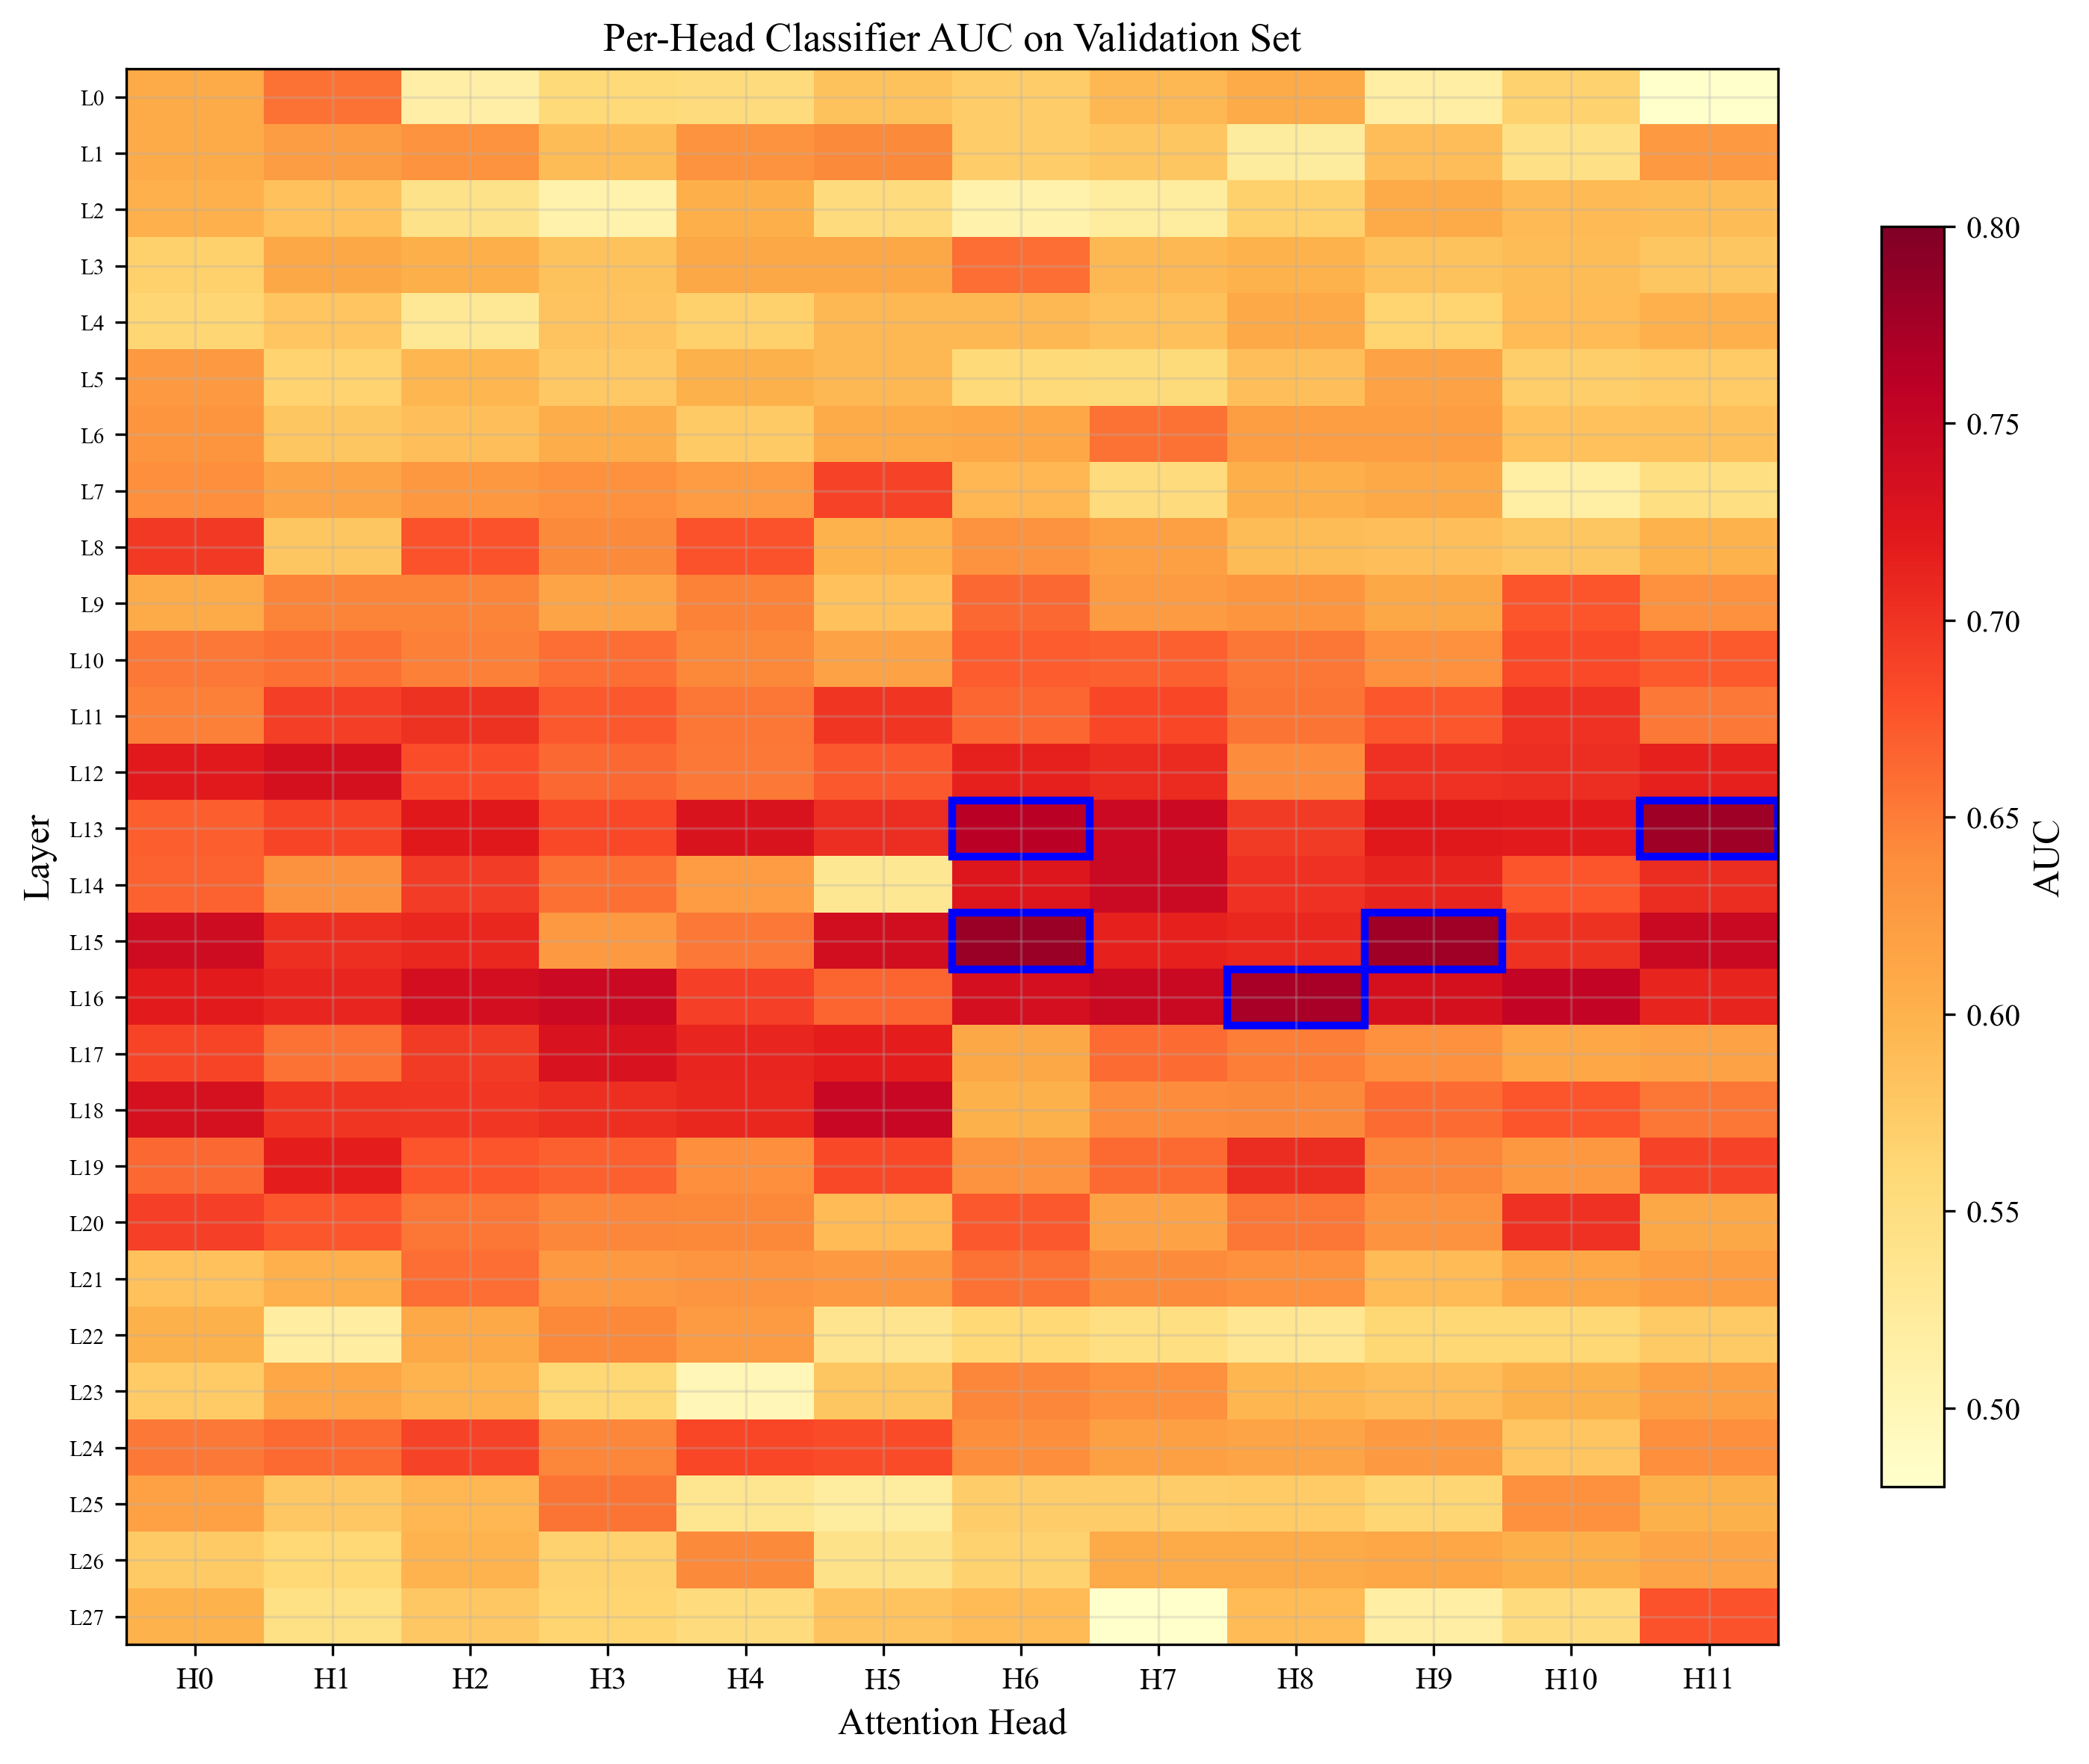
\includegraphics[width=\columnwidth]{processed_datasets/fig_report_4_head_heatmap.png}
    \caption{Per-head classifier AUC heatmap (28 layers $\times$ 12 heads). Blue-bordered cells indicate the top-5 selected heads. High AUC values cluster in layers 13--16.}
    \label{fig:head_heatmap}
\end{figure}

The selected top-5 heads are listed in Table~\ref{tab:top5_heads}. All five heads are located in layers 13--16, consistent with SAPLMA's optimal layer range (Layer 18).

\begin{table}[t]
\centering
\begin{tabular}{clcc}
\toprule
\textbf{Rank} & \textbf{Head} & \textbf{Layer} & \textbf{Val. AUC} \\
\midrule
1 & L15\_H6  & 15 & 0.782 \\
2 & L13\_H11 & 13 & 0.779 \\
3 & L15\_H9  & 15 & 0.778 \\
4 & L16\_H8  & 16 & 0.773 \\
5 & L13\_H6  & 13 & 0.761 \\
\bottomrule
\end{tabular}
\caption{Top-5 attention heads selected by validation AUC. All heads are in layers 13--16.}
\label{tab:top5_heads}
\end{table}

\subsubsection{End-to-End Evaluation}

Table~\ref{tab:end_to_end} compares all methods on the TriviaQA test set (203 samples). Figure~\ref{fig:method_comparison} visualizes the results.

\begin{table}[t]
\centering
\small
\begin{tabular}{lccccc}
\toprule
\textbf{Method} & \textbf{Acc.} & \textbf{Prec.} & \textbf{Rec.} & \textbf{F1} & \textbf{AUC} \\
\midrule
PPL              & .625 & .889 & .098 & .176 & .539 \\
SAPLMA-L18       & .680 & .667 & .439 & .529 & .723 \\
\midrule
Single L15\_H6   & .675 & .579 & .756 & .656 & .755 \\
Single L13\_H11  & .660 & .613 & .463 & .528 & .708 \\
Single L15\_H9   & .680 & .598 & .671 & .632 & .741 \\
Single L16\_H8   & .645 & .590 & .439 & .503 & .704 \\
Single L13\_H6   & .685 & .607 & .659 & .632 & .733 \\
\midrule
Summed-Heads     & \textbf{.710} & \textbf{.676} & .561 & .613 & \textbf{.776} \\
Voting Ensemble  & .685 & .620 & .598 & .609 & .762 \\
\bottomrule
\end{tabular}
\caption{End-to-end hallucination detection on the TriviaQA test set (N=203). The Summed-Heads probe achieves the best AUC (0.776) and Accuracy (0.710).}
\label{tab:end_to_end}
\end{table}

\begin{figure}[t]
    \centering
    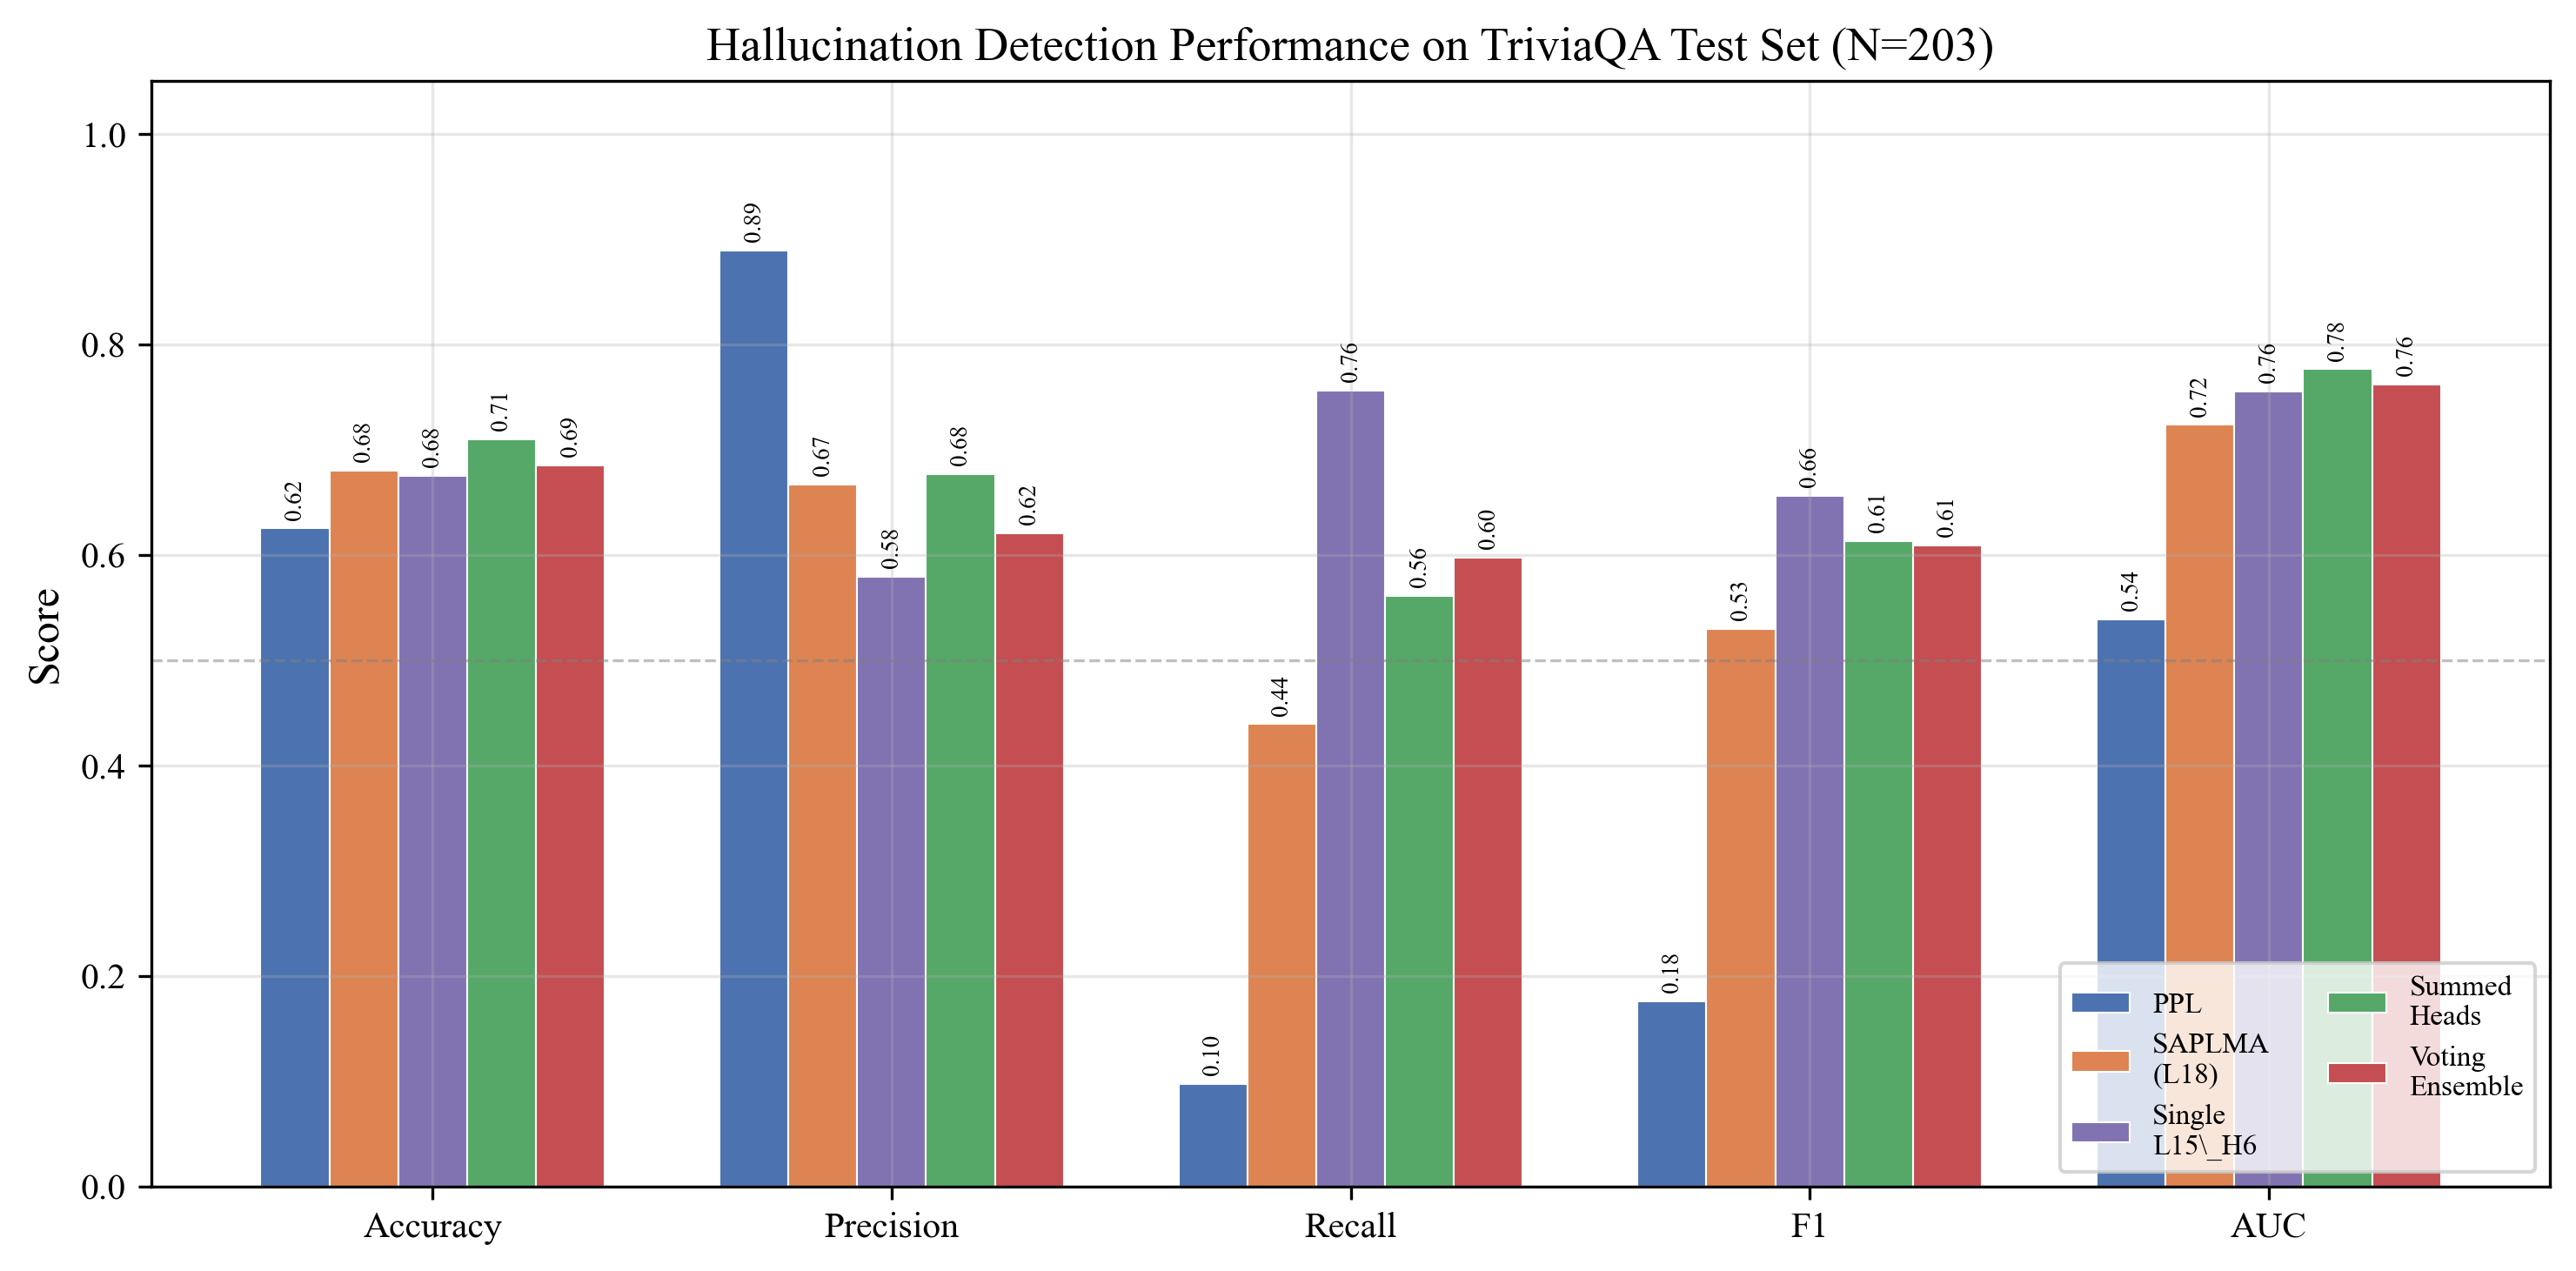
\includegraphics[width=\columnwidth]{processed_datasets/fig_report_5_method_comparison.png}
    \caption{Comparison of all methods on the TriviaQA test set across five metrics. The Summed-Heads probe achieves the best overall performance.}
    \label{fig:method_comparison}
\end{figure}

Key observations:
\begin{itemize}
    \item The \textbf{Summed-Heads probe} (AUC 0.776) surpasses SAPLMA (AUC 0.723) using only 5 of 336 heads' influence vectors, demonstrating that head-level features can be more discriminative than the full hidden state.
    \item \textbf{Feature-level fusion} (Summed-Heads, AUC 0.776) slightly outperforms \textbf{decision-level fusion} (Voting, AUC 0.762), suggesting the head signals are complementary at the feature level.
    \item \textbf{PPL} has near-zero recall (0.098), meaning it almost never correctly identifies hallucinations, despite high precision (0.889). This reflects a strong bias toward predicting ``correct'' for all inputs.
    \item Among single-head probes, \textbf{L15\_H6} achieves the highest recall (0.756) and AUC (0.755), already exceeding the full SAPLMA baseline.
\end{itemize}

\section{Analysis and Discussion}

\subsection{Why Does SAPLMA Outperform PPL?}

The performance gap between SAPLMA (AUC 0.834) and PPL (AUC 0.690) can be attributed to four factors:

\begin{enumerate}
    \item \textbf{Information richness}: PPL uses a single scalar (NLL), while SAPLMA leverages a 1536-dimensional hidden state encoding far richer information.
    \item \textbf{Robustness to surface features}: NLL is influenced by token frequency and sentence length---common token sequences may receive low NLL even when factually incorrect. Hidden states encode more abstract semantic representations.
    \item \textbf{Nonlinear discrimination}: PPL is inherently a linear threshold classifier, while SAPLMA's feedforward probe can learn complex nonlinear decision boundaries.
    \item \textbf{Internal cognitive signals}: Hidden states directly reflect the model's internal representation of the input, including signals about whether the model ``knows'' the statement to be true.
\end{enumerate}

\subsection{The Inverted-U Layer Pattern}

The optimal layer for SAPLMA is Layer 18 (64\% depth), not the final layer. This inverted-U pattern is consistent with the SAPLMA paper's findings for other models. A plausible explanation is that middle-upper layers encode the most abstract and task-relevant representations, while later layers begin to transform these into output-oriented representations optimized for next-token prediction, potentially losing some discriminative information.

\subsection{Why the Last Token?}

The last token's hidden state (AUC 0.835) vastly outperforms earlier positions (AUC $\sim$0.50 for first/second tokens). In autoregressive Transformers, each token's representation attends to all preceding tokens. The last token has ``seen'' the entire statement and thus aggregates the fullest semantic representation. Earlier tokens lack this global context.

\subsection{Head-Level Interpretability}

The concentration of high-performing heads in layers 13--16 (Figure~\ref{fig:head_heatmap}) provides interpretable evidence that hallucination-relevant information is localized in specific model components. This is consistent with findings on factual knowledge localization \citep{meng2022locating} and circuit analysis \citep{olah2020zoom}. The fact that only 5 of 336 heads suffice to surpass SAPLMA suggests that truth-discriminative signals are highly concentrated rather than uniformly distributed.

\subsection{Feature-Level vs Decision-Level Fusion}

The slight advantage of Summed-Heads (AUC 0.776) over Voting (AUC 0.762) suggests that the top-5 heads capture complementary aspects of the truth/hallucination distinction, and that combining their signals at the feature level allows the probe to learn richer joint patterns than majority voting at the decision level.

\section{Limitations}

Our study has several limitations. First, the true/false dataset uses a constrained statement format that may not fully represent the diversity of real-world hallucinations. Second, the TriviaQA-based evaluation relies on fuzzy string matching for auto-labeling, which introduces annotation noise. Third, we evaluate on a single model (Qwen2-1.5B); generalization to larger models and different architectures remains to be verified. Fourth, the per-head probe method requires a forward pass through the model for feature extraction, which adds computational overhead compared to PPL. Finally, our voting ensemble uses a simple majority rule; more sophisticated fusion strategies may yield further improvements.

\section{Conclusion}

We conducted a systematic three-stage study of hallucination detection using the internal states of Qwen2-1.5B. Our key findings are:

\begin{enumerate}
    \item SAPLMA (AUC 0.834) significantly outperforms PPL (AUC 0.690), confirming that hidden states contain richer truth-discriminative information than output probabilities.
    \item The optimal detection layer is Layer 18 (64\% depth), not the final layer, and the last token position is critical for effective detection.
    \item A novel per-head probe method, using only 5 of 336 attention heads' influence vectors, achieves AUC 0.776 on a TriviaQA test set---surpassing the full SAPLMA baseline (AUC 0.723) with 300$\times$ fewer features.
    \item The most discriminative heads cluster in layers 13--16, providing interpretable evidence for the localization of hallucination-related signals in Transformer models.
\end{enumerate}

These results demonstrate that interpretable, head-level probes can rival or exceed full-hidden-state methods for hallucination detection, opening new directions for efficient and explainable detection systems.

\section*{Acknowledgments}

We thank the anonymous reviewers for their valuable feedback. This work was completed as a course project for Natural Language Processing.

\bibliography{custom}

\end{document}
